\chapter{Contesto}
\label{chap:contesto}

\section{Il simulatore Alchemist}
\label{sec:alchemist}

Alchemist~\cite{alchemist} è un simulatore di sistemi complessi, scritto in Java e
Kotlin, nato alla fine del 2010 come sottoprodotto del progetto europeo SAPERE e
mantenuto da allora come progetto open source da Danilo Pianini e collaboratori presso
il Dipartimento di Informatica dell'Università di Bologna.

In Alchemist una simulazione è composta da un \emph{environment}, lo spazio in cui
vivono i \emph{nodi}. Ciascun nodo è un contenitore di \emph{molecole} (identificatori,
l'equivalente di un nome di variabile) a cui sono associate \emph{concentrazioni},
i valori che esse assumono, e di \emph{reazioni}, gli eventi che ne modificano lo stato
nel tempo. Il metamodello è mostrato nella \Cref{fig:metamodel}.

\begin{figure}[H]
    \centering
    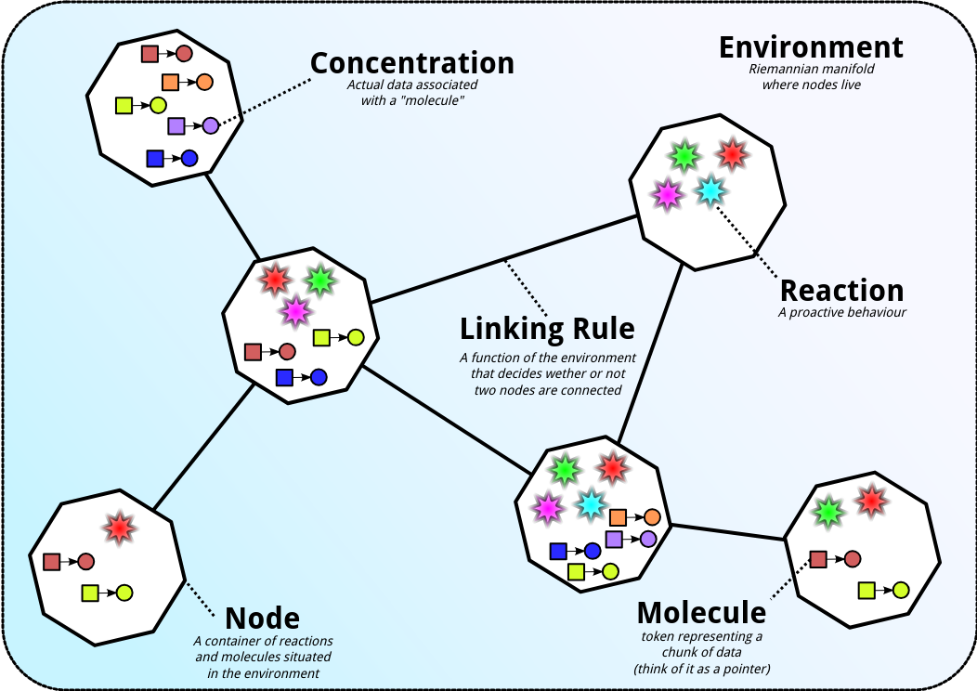
\includegraphics[width=\linewidth]{figures/alchemist/metamodel.png}
    \caption[Il metamodello di Alchemist]{Il metamodello di Alchemist. Immagine tratta dal sito ufficiale del simulatore~\protect\footnotemark.}
    \label{fig:metamodel}
\end{figure}
\footnotetext{Spiegazione del metamodello di Alchemist: \url{https://alchemistsimulator.github.io/explanation/metamodel/}.}

Alchemist è impiegato come strumento in diversi lavori di ricerca.
Ad esempio, in~\cite{aguzzi2022dynamic} è stato usato per simulare, sull'area urbana di Toronto,
un sistema \ac{IoT} decentralizzato di allerta alluvionale: i valori di pioggia
misurati da una rete di pluviometri, ricavata da dati reali, vengono aggregati
in modo distribuito per pre-allertare le stazioni dei vigili del fuoco prossime alle
zone a rischio. In~\cite{audrito2021optimal} il simulatore costituisce invece l'intero
apparato sperimentale del lavoro: viene utilizzato sia per confrontare algoritmi
decentralizzati di raccolta e aggregazione dei dati su reti di dispositivi mobili,
esplorando parametri quali densità, diametro della rete e velocità
di movimento, sia per uno studio in cui gli stessi algoritmi vengono applicati
al tracciamento di una folla in un parco cittadino.

Le sezioni che seguono si limitano agli elementi necessari a collocare il lavoro
descritto in questa tesi: la nozione di layer, il modo in cui il tempo di simulazione è
reso accessibile ai componenti, il supporto geospaziale già disponibile e il sistema di
caricamento delle simulazioni da file YAML.

\subsection{Il motore di simulazione}
\label{subsec:alchemist-lifecycle}

Una simulazione Alchemist nasce da una configurazione dichiarativa
(Sezione~\ref{subsec:alchemist-loader}), a partire dalla quale sono istanziati
l'environment, i layer, i nodi con le rispettive reazioni e contenuti. Il modello
che ne risulta descrive lo stato iniziale della simulazione.

A metterlo in esecuzione è il motore, un simulatore a eventi discreti la cui implementazione si
fonda sul \emph{Next Reaction Method} di Gibson e Bruck~\cite{gibson}. Il motore
procede per passi: a ogni passo viene selezionata, fra tutte le reazioni
schedulate, quella il cui istante di esecuzione è il più vicino; il tempo di simulazione
assume tale istante; la reazione viene eseguita, modificando lo stato del modello;
infine vengono rischedulate le reazioni la cui esecuzione dipende da quella appena
avvenuta. Il tempo non avanza quindi a passi costanti, ma per salti da un evento al
successivo, e fra due eventi consecutivi lo stato del modello resta invariato.

Il punto d'ingresso del motore è la \texttt{Simulation}, che custodisce il tempo di simulazione
corrente ed espone i comandi per avviare, sospendere e arrestare l'esecuzione. Lo stato
in cui essa si trova è descritto da un insieme predefinito di valori, dall'inizializzazione
alla terminazione, ed è interrogabile in qualunque momento.

\subsection{Il concetto di \emph{layer}}
\label{subsec:alchemist-layer}

Le molecole e le concentrazioni descrivono lo stato interno dei singoli nodi. Alcune
grandezze, però, non appartengono ad alcun nodo in particolare: sono proprietà
dell'ambiente stesso, definite in ogni suo punto indipendentemente dal fatto che vi si
trovi o meno un nodo a percepirle. La temperatura, l'intensità luminosa, la
concentrazione di un inquinante in atmosfera sono esempi di questo tipo: un nodo che
si muove nello spazio ne osserva valori diversi non perché il proprio stato sia
cambiato, ma perché è cambiata la sua posizione.

Alchemist modella queste grandezze attraverso il concetto di \emph{layer}: una
sovrapposizione di dati distribuita sull'ambiente, associata a una molecola e
interrogabile da qualunque punto dello spazio. Formalmente, un \texttt{Layer<T, P>} è
una funzione che associa a ogni posizione di tipo \texttt{P} dell'environment un
valore di tipo \texttt{T}. L'interfaccia si riduce a un solo metodo:

\lstinputlisting[language=Java,label={lst:layer-interface}]{listings/Layer.java}

Un nodo può quindi interrogare un
layer con la propria posizione corrente e ottenere il valore che il layer associa a
quel punto, usandolo per esempio come stimolo a cui reagire.

Le implementazioni preesistenti in Alchemist realizzano però tutte layer
che producono valori sintetici, determinati da una regola fissata alla costruzione, come
\sloppypar{\texttt{BidimensionalGaussianLayer}}, che descrive una distribuzione
gaussiana bidimensionale centrata su un punto. Queste realizzazioni sono adeguate a
rappresentare fenomeni il cui comportamento varia rispetto a una formula,
ma non un fenomeno misurato: i dati ambientali reali non sono
espressi da una funzione, bensì campionati su griglie spaziali a risoluzione
finita, disponibili solo in corrispondenza di determinati istanti e distribuiti in
formati binari specialistici.

\subsection{Il tempo di simulazione}
\label{subsec:alchemist-time}

Alchemist rappresenta l'istante corrente di una simulazione come un valore scalare di tipo
\texttt{Time}, privo di un'unità di misura intrinseca: la sua interpretazione è una convenzione
lasciata al modellista della simulazione (ad esempio secondi, ore, giorni), non
un vincolo imposto dal simulatore; il suo tempo parte da zero e cresce con l'avanzare degli eventi.

Il tempo di simulazione appartiene al motore, che viene creato solo quando il modello è
già completo. Un componente, nel momento in cui viene costruito, non ha quindi ancora
alcun tempo da leggere: può ottenerlo soltanto durante l'esecuzione, interrogando la
\texttt{Simulation} attraverso l'environment.

Un layer, in particolare, riceve come unico argomento la posizione da cui è interrogato
(Sezione~\ref{subsec:alchemist-layer}): se il valore che restituisce dipende anche dal
tempo, è il layer stesso a doverselo procurare per questa via.

\subsection{Il supporto geospaziale preesistente}
\label{subsec:alchemist-osm}

Alchemist offre un supporto già maturo per simulazioni su cartografia
reale: un \texttt{OSMEnvironment} può caricare estratti di OpenStreetMap e collocare i
nodi al suo interno, vincolandone il movimento a una rete stradale e delegando il calcolo
dei percorsi a GraphHopper~\footnote{Motore di calcolo dei percorsi GraphHopper: \url{https://www.graphhopper.com/}.}.
Le posizioni in questi ambienti sono espresse come \texttt{GeoPosition}, coppie di
latitudine e longitudine. È questa asimmetria che fa nascere il problema affrontato in questa tesi:
un simulatore capace di collocare e muovere con precisione i propri nodi nello spazio geografico reale, ma
non dotato di un modo per far percepire loro misurazioni campionate nello spazio.

\subsection{Il caricamento delle simulazioni da YAML}
\label{subsec:alchemist-loader}

Una simulazione Alchemist si specifica tipicamente in modo dichiarativo, in un file YAML
che indica, per ciascun componente, il nome della classe che lo implementa e i parametri
con cui costruirlo. Questo meccanismo, basato sulla reflection, non è un semplice dettaglio
di configurazione: i vincoli che impone hanno condizionato la forma di ogni classe destinata
a essere istanziata da YAML.

Il layer gaussiano introdotto nella Sezione~\ref{subsec:alchemist-layer} è costruito dal
seguente costruttore, di sei parametri, di cui il primo (\texttt{baseline}) e l'ultimo
(\texttt{sigmaY}) sono opzionali:

\lstinputlisting[language=Kotlin,label={lst:bidimensional-gaussian-layer-kotlin}]{listings/BidimensionalGaussianLayer.kt}

Il loader individua la classe indicata dalla chiave \texttt{type}, ne seleziona un
costruttore compatibile con gli argomenti forniti e lo invoca tramite reflection. Nella
forma più diretta, i parametri sono specificati posizionalmente:

\lstinputlisting[language=YAML,label={lst:bidimensional-gaussian-layer}]{listings/bidimensional.yml}

la chiave \texttt{molecule} indica la molecola a cui il layer viene associato
nell'environment, mentre \texttt{parameters} elenca gli argomenti del costruttore. I
quattro valori forniti vengono associati, nell'ordine, a \texttt{centerX},
\texttt{centerY}, \texttt{norm} e \texttt{sigmaX}, mentre \texttt{baseline} e
\texttt{sigmaY} assumono i rispettivi valori di default. La costruzione equivalente, se
scritta direttamente in Kotlin, sarebbe:

\lstinputlisting[language=Kotlin,label={lst:bidimensional-gaussian-equivalent}]{listings/bidimensional-equivalent.kt}

Che i parametri opzionali possano essere omessi non è però una capacità del loader: gli
argomenti di default sono una nozione di Kotlin, invisibile alla reflection della \ac{JVM}, e a
renderli accessibili è l'annotazione \texttt{@JvmOverloads} presente nel
costruttore, la quale istruisce il compilatore a generare costruttori aggiuntivi, ottenuti
rimuovendo i parametri dotati di default a partire dall'ultimo. Ne
discende che da YAML si può omettere soltanto un
suffisso della lista dei parametri opzionali. Per specificare \texttt{sigmaY} occorrerebbe
fornire anche \texttt{baseline}, che lo precede.
L'ordine in cui i parametri opzionali sono dichiarati non è quindi indifferente.

Oltre che per via posizionale, i parametri possono essere specificati anche tramite il
nome dell'argomento a cui si riferiscono:

\lstinputlisting[language=YAML,label={lst:bidimensional-gaussian-layer-named}]{listings/bidimensional-names.yml}

Questa forma elimina l'ambiguità sull'ordine e rende esplicito a quale parametro ciascun
valore si riferisca, ma resta soggetta al vincolo appena descritto.

Non tutti i parametri, infine, provengono dal file YAML: le entità già costruite al momento
dell'istanziazione, fra cui l'environment stesso, sono iniettate automaticamente laddove un
parametro ne dichiari il tipo, e non compaiono quindi fra quelli dichiarati nella
configurazione.

L'istanza risultante viene registrata, nell'environment, in corrispondenza della molecola
indicata dalla chiave \texttt{molecule} (\texttt{moleculeName}).

\section{Il programma Copernicus e i suoi servizi di dati}
\label{sec:copernicus}

Copernicus~\footnote{Il programma Copernicus: \url{https://www.copernicus.eu/it}.}
è il programma di osservazione della Terra dell'Unione Europea, articolato in
servizi tematici. Fra questi, il \ac{CEMS} %\footnote{\url{https://emergency.copernicus.eu/}}
fornisce informazioni geospaziali a supporto della gestione di emergenze ed eventi di
protezione civile, ed è il servizio da cui ha preso avvio il progetto descritto in questa
tesi.

L'accesso programmatico ai dati non è però organizzato per servizio: avviene attraverso
una famiglia di \emph{data store} gestiti dall'\ac{ECMWF}~\footnote{Centro Europeo per le previsioni meteorologiche a medio termine: \url{https://www.ecmwf.int/}}
e costruiti sulla stessa
infrastruttura software, differenziati per host e per il dominio dei dataset che
espongono:

\begin{itemize}
    \item il \ac{CDS}, data store del \ac{C3S}, che ospita fra gli altri ERA5, la
    rianalisi climatica globale prodotta da \ac{ECMWF};
    \item l'\ac{EWDS}, data store del \ac{CEMS}, che ospita i dataset di \ac{EFAS} e
    \ac{GloFAS}, sistemi di allerta alluvionale rispettivamente a scala europea e
    globale, e quelli relativi agli incendi boschivi;
    \item l'\ac{ADS}, data store del \ac{CAMS}, relativo a composizione atmosferica,
    qualità dell'aria, gas serra e radiazione solare.
\end{itemize}

I tre condividono la stessa infrastruttura, per cui un unico
client è sufficiente a interrogarli tutti, e la differenza si riduce all'host e al
catalogo dei dataset disponibili.

L'autenticazione verso i tre data store avviene tramite un unico token \ac{ECMWF}:
la stessa identità è valida su \ac{CDS}, \ac{EWDS} e \ac{ADS}, e viene letta da un file di configurazione
locale nel formato \texttt{.cdsapirc}~\footnote{Struttura del file \texttt{.cdsapirc}: \url{https://cds.climate.copernicus.eu/how-to-api}},
lo stesso adottato dal client Python ufficiale di \ac{ECMWF}.

\section{Formati e convenzioni per dati raster geospaziali}
\label{sec:formati-raster}

I dataset offerti dai tre data store descritti precedentemente sono forniti,
a seconda del dataset e della selezione effettuata in fase di richiesta, in due
formati binari pensati per la memorizzazione di dati geospaziali multidimensionali
campionati su una griglia: \ac{GRIB} e \ac{NetCDF}. Entrambi distribuiscono i valori
di una o più grandezze fisiche su assi di latitudine, longitudine e tempo, dove l'asse temporale
è una successione di istanti assoluti associati a un calendario di riferimento. Nel
dettaglio:

\begin{itemize}
\item \ac{GRIB}, distribuito dai data store nelle versioni GRIB1 e GRIB2, è uno standard
    binario definito dalla \ac{WMO}, con l'obiettivo di
    trasmettere in modo efficiente i grandi volumi di dati prodotti dai modelli
    meteorologici. Un file \ac{GRIB} non è autosufficiente dal punto di vista semantico:
    la grandezza fisica contenuta è identificata da codici numerici, il cui significato è
    definito da tabelle esterne, standard o specifiche del centro meteorologico di
    origine. Ad esempio, nella tabella 128 di \ac{ECMWF} il codice 167 identifica la
    temperatura registrata a due metri dal suolo~\footnote{Tabella ECMWF per i file GRIB che esprimono la temperatura a due metri dal suolo: \url{https://codes.ecmwf.int/grib/param-db/167}},
    ma la corrispondenza fra codice e
    grandezza fisica non è ricavabile dal solo contenuto del file;
\item \ac{NetCDF}, distribuito dai data store nelle versioni NetCDF3 e NetCDF4, è un formato
    sviluppato e mantenuto da Unidata, un programma comunitario dell'\ac{UCAR},
    orientato all'accesso e alla condivisione di dati scientifici
    multidimensionali. A differenza di \ac{GRIB}, un file \ac{NetCDF} è
    autodescrittivo: nomi delle variabili, unità di misura e altri metadati
    sono incorporati nel file stesso. Il formato di per sé impone però una
    struttura minima; per questo la comunità scientifica ha definito
    convenzioni che ne regolano il contenuto: nome e ordine delle dimensioni,
    attributi obbligatori, semantica degli assi. La più diffusa, e adottata
    dagli store di riferimento, è la convenzione \ac{CF}~\cite{cf_conventions}, \Cref{fig:netcdf-structure}.
\end{itemize}

\begin{figure}[H]
    \centering
    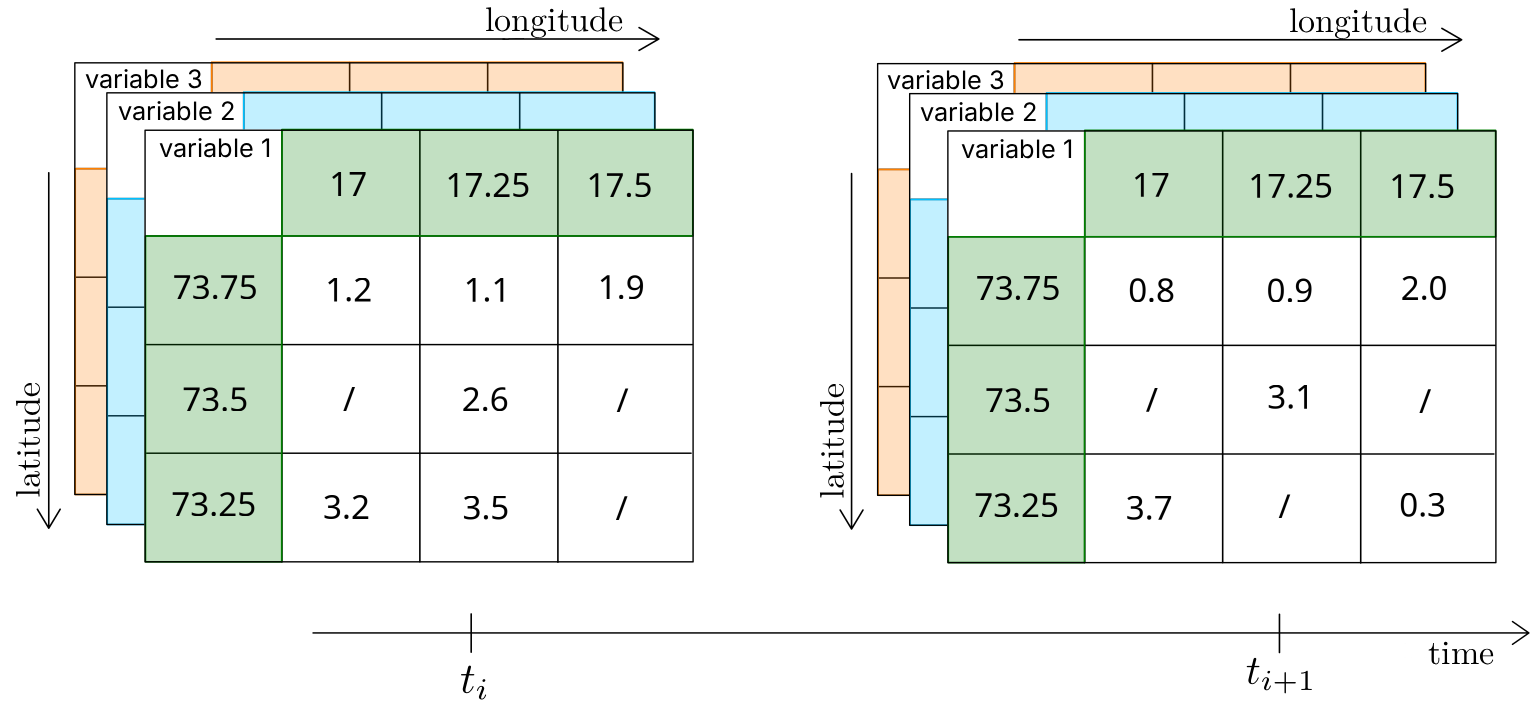
\includegraphics[width=0.75\linewidth]{figures/netcdf-file-structure.png}
    \caption[Struttura CF di un file NetCDF]{Struttura CF di un file NetCDF. Immagine tratta da \cite{simulating_complexity_netcdf}.}
    \label{fig:netcdf-structure}
\end{figure}

Un aspetto comune ai due formati riguarda la rappresentazione dei valori mancanti, che nei
dataset forniti dai data store non è un caso raro: le misure di portata fluviale, ad esempio,
sono definite solo in corrispondenza dei corsi d'acqua, e lasciano prive di valore tutte
le altre celle della griglia. 
%In un file \ac{NetCDF} conforme alle convenzioni \ac{CF}
%l'assenza di un valore è segnalata dall'attributo \texttt{\_FillValue} o \texttt{missing\_value}:
%un valore riservato, che le librerie di lettura riconoscono come indicatore di dato mancante.~\cref{fig:netcdf-structure}

%In un file \ac{GRIB} lo stesso ruolo è svolto da una sezione dedicata,
%la \emph{bitmap section}, che indica punto per punto della griglia se il valore
%corrispondente sia presente. Il modo in cui queste due rappresentazioni vengono
%ricondotte a un'unica convenzione interna è
%discusso nel Capitolo~\ref{chap:implementazione}.

Un secondo aspetto, comune a entrambi i formati, riguarda la nozione di
\emph{griglia raster}. Nella sua forma più diffusa, una griglia raster è
definita dal prodotto cartesiano di un asse di latitudini e uno di longitudini,
indipendenti fra loro: ogni cella è quindi individuabile con una coppia di
coordinate geografiche. Questa non è però l'unica struttura possibile.
Alcuni dei dataset distribuiti dai data store sono definiti su una griglia nativa espressa in
una proiezione cartografica, ad esempio \ac{LAEA}, non riconducibile al prodotto
cartesiano di due assi indipendenti di latitudine e longitudine.

Un punto rilevante, con conseguenze dirette sulle scelte implementative,
riguarda la spaziatura degli assi. La convenzione \ac{CF} richiede che
latitudine e longitudine siano strettamente monotone, ma non equispaziate, e
sull'asse temporale il vincolo non è più forte: un dataset può
contenere misurazioni a intervalli di tempo non regolari.
Nel caso di \ac{GRIB} la questione non si pone nemmeno in
termini di convenzione, dal momento che un file è una successione di
griglie indipendenti, ciascuna con il proprio istante di validità: nulla
nel formato impone che l'insieme risultante sia ordinato, né tanto meno
regolare.

\section{Il paradigma OGC API Processes}
\label{sec:ogc-api-processes}

Le richieste di dati verso i tre data store Copernicus sono operazioni di durata variabile,
da qualche secondo a diverse decine di minuti in base all'entità della richiesta, e vengono
quindi gestite in modo asincrono: il client sottomette una richiesta, ottiene l'indirizzo a
cui interrogarne lo stato, e lo interpella periodicamente fino al completamento
dell'elaborazione.

Lo schema è descritto, a livello di standard, da \ac{OGC} in \emph{OGC API - Processes -
Part 1: Core}~\cite{ogc_api_processes_core}, che specifica un'interfaccia REST per
l'esecuzione di elaborazioni remote e per il recupero dei relativi risultati. Il ciclo di
vita di un job si articola in tre fasi:
la sottomissione, tramite una richiesta \texttt{POST} all'endpoint di esecuzione del
processo; l'interrogazione dello stato, il cui indirizzo lo standard prescrive sia
comunicato al client nell'intestazione \texttt{Location} della risposta alla
sottomissione; e il recupero dei risultati, disponibile una volta che il job ha raggiunto
uno stato terminale. Lo standard definisce inoltre l'insieme degli stati che un job può
assumere durante l'elaborazione, distinguendo quelli intermedi da quelli terminali, ai
quali è associata la disponibilità dei risultati o della descrizione dell'errore.

Ogni risposta include, oltre ai dati che rappresenta, un vettore \texttt{links}. Ciascun
collegamento è accompagnato da una relazione (\texttt{rel}), un'etichetta che ne dichiara
il significato: quale risorsa il collegamento raggiunga e in che rapporto stia con quella
corrente. Lo standard stabilisce quali relazioni usare per le risorse che definisce, ad
esempio \texttt{status} per lo stato di un job, e consente alle implementazioni di
aggiungere collegamenti propri, oltre a quelli previsti.

Per gli errori, lo standard raccomanda, senza imporlo, il formato \emph{Problem Details}
definito dalla RFC 7807~\cite{rfc7807}, che uniforma la struttura del corpo delle risposte
di errore e la rende interpretabile.

I data store \ac{ECMWF} si ispirano a questo paradigma, ma se ne discostano su più punti,
alcuni dei quali non documentati. Tali scostamenti hanno determinato scelte
implementative del sottosistema di acquisizione, e sono discussi nel Capitolo ~\ref{chap:implementazione}.
\emph{\textbf{("??" = link al capitolo di implementazione, attualmente assente)}}